\documentclass[12pt,preprint]{aastex61}

%\usepackage{graphicx}
%\usepackage{subfigure}
%\usepackage{amsmath}
%\usepackage{array,multirow}


\begin{document}

\title{Red wine quality dataset: analysis} 

  \author{Remschira}

\begin{abstract}

  The wine quality dataset \citep{Cortez_etal_2009} contains
physicochemical and sensory information for red and white variants of
the Portuguese ``Vinho Verde'' wine. The goal of this project is to
use machine learning and data analysis methods to predict accurately
the quality of a red wine based on its physicochemical makeup using
the red wine dataset. The quality of the wine is measured by a score
that takes integer values between 0 and 10. We apply several
regression and classification methods to the dataset in order to
determine which algorithm provides the most accurate predictions. For
each of the tested machine learning algorithms, we search the
hyperparameter space to find where it performs best on our accuracy
measures. As part of our accuracy tests, we include 5-fold cross
validation on the training dataset. We incorporate outlier detection
and removal to understand the influence of potentially anomalous data
on the results. To aid the visualization of the data we use Principal
Component Analysis to project the data into two- and
three-dimensions. We find that the Random Forest classifier performs
best on our accuracy measures.

% We do
% not find a significant difference between applying the Random Forest
% classifier on the full dataset versus the dataset with outliers
% removed.

\end{abstract}
  

\section{Outline\label{Outline}}


The outline of this write-up is as follows. In Section~\ref{viz}, we
visualize the distribution of the data and look for correlations
between the physicochemical characteristics or features of the
wine. Principal Component Analysis (PCA) is applied to see how much
variance is explained by each principal component of the
data. Section~\ref{outlier} addresses our implementation of outlier
detection methods. The two algorithms we study are known as
``Elliptical Envelope''
(\texttt{sklearn.covariance.EllipticalEnvelope}) and ``Isolation
Forest'' (\texttt{sklearn.ensemble.IsolationForest}).\footnote{This
project makes use of the sklearn Python library
\citep{Pedregosa_etal_2011}.}  Section~\ref{classifiers} provides an
outline of the various machine learning algorithms we apply to the
dataset and reports the results of each method under our performance
measures.


% Section 4 provides an outline of the various machine
% learning algorithms we apply to the dataset and provides a
% description of how we measure the performance of each algorithm.
% Section 5 reports the results of each method. We then compare the two
% top performing algorithms (Section 6). Section 7 summarizes the
% results of the Random Forest classifier on the full dataset to the
% results obtained on (1) the data with outliers removed and (2) the
% data projected onto its three principal components. We provide our
% conclusions in Section 8. 


\section{Data visualization \label{viz}}

The red wine dataset contains data for 1599 wines. Each wine is
characterized by 11 different physicochemical features and is scored
on a 0 - 10 integer scale.  Figure~\ref{FIG-Data-Histo} shows the
distribution of each variable. The horizontal axis shows that the
variables are on different scales, which suggests the need to shift
and scale each variable. Additionally, a by-eye inspection of the
distributions suggests that some of the variables are approximately
normally distribution (e.g.  the ``density'' and ``pH'' variables). To
check this we could use one of the popular tests of normality, such as
the chi-square test. However, any test of normality for our large
sample will likely fail because no variable in the dataset is exactly
normally distributed. Moreover, although the pH variable looks
normally distributed, for example, this may be an artifact of the
binning used to make the histogram.

The boxplot for each variable is shown in
Figure~\ref{FIG-Data-Box}. The ``free sulfur dioxide'' and ``total
sulfur dioxide'' features have a much wider range than the other
variables. However, this is likely due to each variable being
expressed in different units. To test this, we present the box plot
graph in Figure~\ref{FIG-Scaled-Data-Box} for the scaled version of
the training data for the wine features.

We now would like to visualize the correlation between the wine
variables. We do so with a ``heat map'' (Figure~\ref{FIG-HeatMap})
(idea from \citealp{Li_2017}).  In the case of a set of variables that
are $100\%$ independent, all off-diagonal entries in the heatmap would
be zero. That is, the correlation between any two of the variables
would be zero, assuming non-zero standard deviations. This is not the
case for our dataset.  However, this is not surprising as one expects
correlations between the characteristics of a wine.

Our dataset can be thought of as a cloud of points in 11-dimensions
(there are 11 features) and each point is labeled by that particular
wine's score. Principal component analysis (PCA)
(\texttt{sklearn.decomposition.PCA}) finds in which direction the
variation is greatest in the cloud of data points. This direction is
the first principal component of the dataset. The procedure also finds
the direction, perpendicular to the first component, along which the
variation is second greatest. This is the second principal
component. The procedure continues for all 11 dimensions of the
dataset. Through PCA, our dataset gets expressed in its principal
components that are linearly uncorrelated to each other. Each
component accounts for a certain amount of the variation in the
dataset. This is visualized in Figure~\ref{FIG-Explained-Variance}
(idea for plot from \citealp{Hong} and \citealp{Raschka_2015}).  One
can project the PCA-transformed dataset into lower dimensions.
Figures~\ref{FIG-PCA-2D} and \ref{FIG-PCA-3D} show the data projected
into two and three dimensions \citep{Raschka_2015}.



 %%%%%%%%%%%%%%%%%%%%%%%% FIG-Data-Histo %%%%%%%%%%%%%%%%%%%%%%%%
 \begin{figure}
 \centering 
 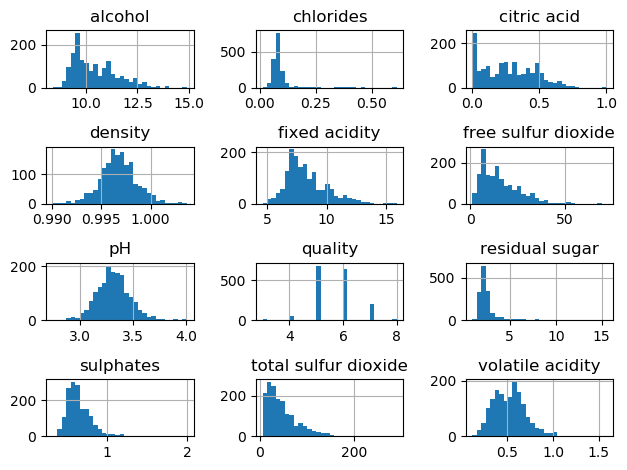
\includegraphics[angle=0,width=130mm]{../output/allDataHisto.png}
 \caption{
   Binned distributions of the variables in the red wine dataset ordered alphabetically.
   ``Quality'' is the dependent variable and is categorical. All other variables
   are the physical attributes of the wines.
 \label{FIG-Data-Histo}}
 \end{figure}


 %%%%%%%%%%%%%%%%%%%%%%%% FIG-Data-Box %%%%%%%%%%%%%%%%%%%%%%%%
 \begin{figure}
 \centering 
 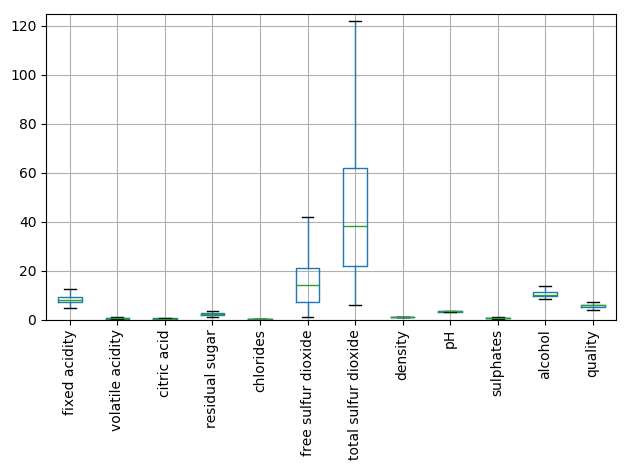
\includegraphics[angle=0,width=130mm]{../output/allDataBoxPlot.png}
 \caption{
   The unscaled distributions in boxplot-form of the variables in the red wine dataset. 
 \label{FIG-Data-Box}}
 \end{figure}


 %%%%%%%%%%%%%%%%%%%%%%%% FIG-Scaled-Data-Box %%%%%%%%%%%%%%%%%%%%%%%%
 \begin{figure}
 \centering 
 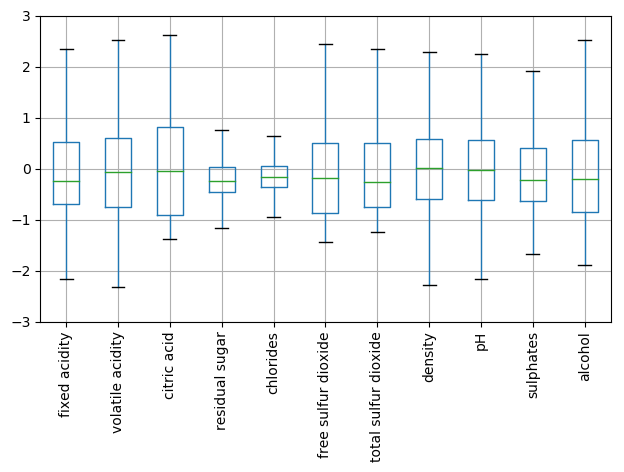
\includegraphics[angle=0,width=130mm]{../output/scaledTrainDataBoxPlot.png}
 \caption{
   The scaled distributions in boxplot-form of the wine features in the training set.
 \label{FIG-Scaled-Data-Box}}
 \end{figure}


 %%%%%%%%%%%%%%%%%%%%%%%% FIG-HeatMap %%%%%%%%%%%%%%%%%%%%%%%%
 \begin{figure}
 \centering 
 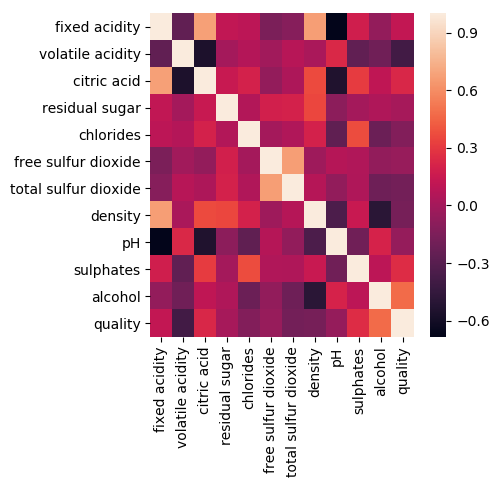
\includegraphics[angle=0,width=130mm]{../output/feature_heatMap.png}
 \caption{
   A heatmap visualization of the correlation matrix for the variables in the wine dataset,
   produced using the Seaborn Python library.
 \label{FIG-HeatMap}}
 \end{figure}

 %%%%%%%%%%%%%%%%%%%%%%%% FIG-Explained-Variance %%%%%%%%%%%%%%%%%%%%%%%%
 \begin{figure}
 \centering 
 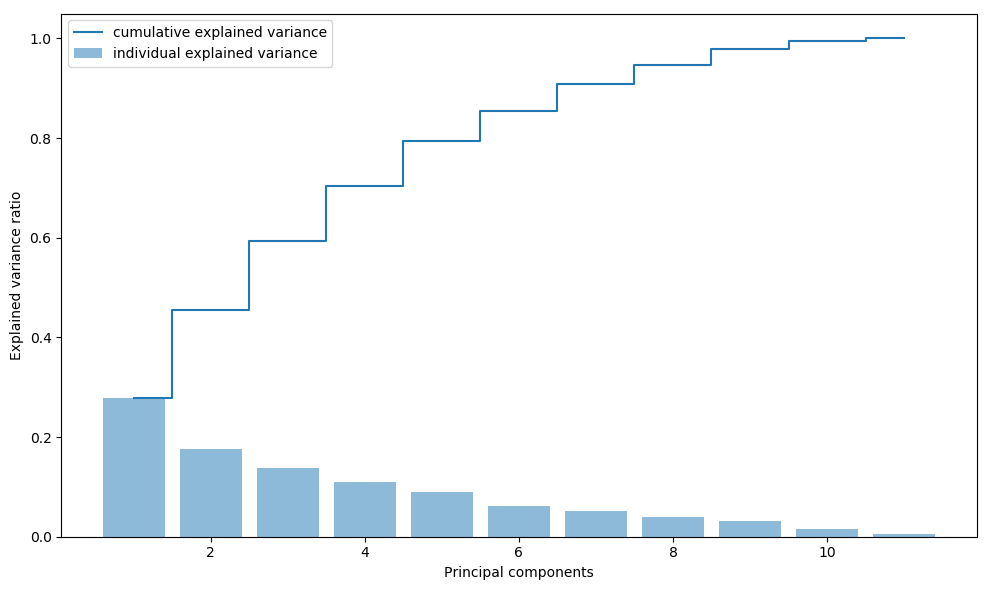
\includegraphics[angle=0,width=130mm]{../output/explainedVariance.png}
 \caption{
   The individual amount of variance explained by each principal component along
   with the cumulative explained variance.
 \label{FIG-Explained-Variance}}
 \end{figure}

 %%%%%%%%%%%%%%%%%%%%%%%% FIG-PCA-2D %%%%%%%%%%%%%%%%%%%%%%%%
 \begin{figure}
 \centering 
 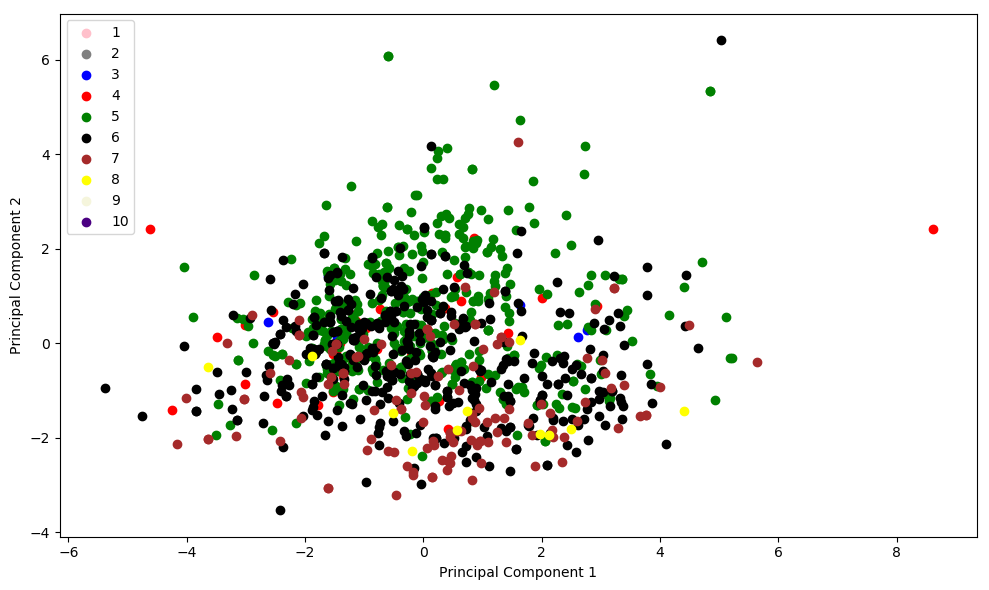
\includegraphics[angle=0,width=130mm]{../output/PCA_2D.png}
 \caption{
   The projection of the PCA-transformed dataset into two dimensions. Each
   color represents a different quality score.
 \label{FIG-PCA-2D}}
 \end{figure}


 %%%%%%%%%%%%%%%%%%%%%%%% FIG-PCA-3D %%%%%%%%%%%%%%%%%%%%%%%%
 \begin{figure}
 \centering 
 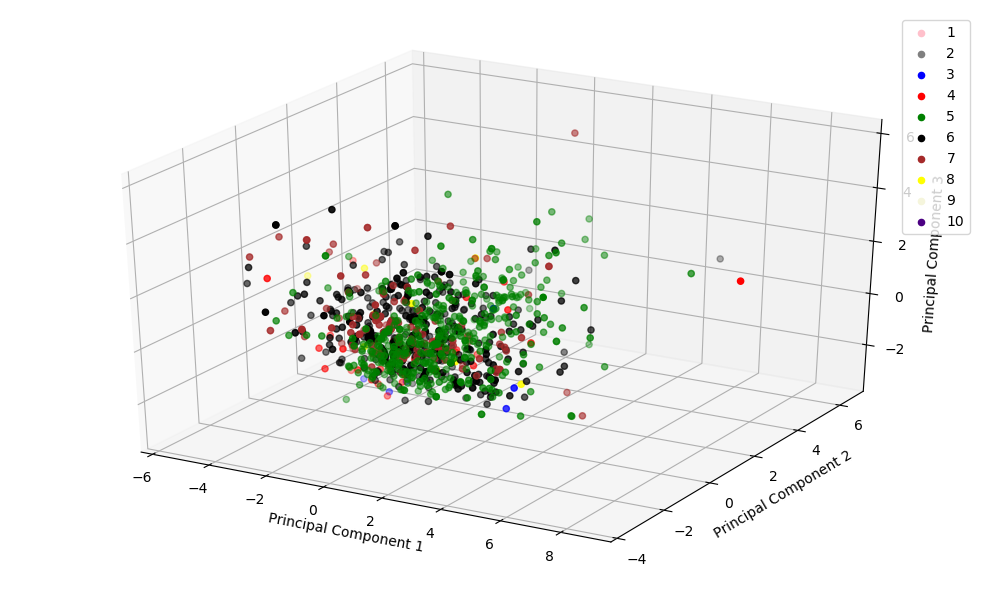
\includegraphics[angle=0,width=130mm]{../output/PCA_3D.png}
 \caption{
   Same as Figure~\ref{FIG-PCA-2D} but now the data is projected into three dimensions.
 \label{FIG-PCA-3D}}
 \end{figure}


 \section{Outlier detection \label{outlier}}

 Here we discuss our implementation of two different outlier detection
methods and discuss how the results of the two methods applied to the
wines dataset differ. The first method we will address is known in the
sklearn library as \texttt{sklearn.covariance.EllipticalEnvelope}. The
method assumes the data to be Gaussian distributed and uses robust
covariance estimation.  The algorithm fits an ellipse to the data and
leaves out data points that are sufficiently removed from the central
mode (see the scikit learn webpage entitled ``Novelty and Outlier
Detection''). The method takes as a parameter the contamination
fraction, which is the fraction of outliers in the
dataset. Figure~\ref{FIG-Ell-Outliers-PCA-3D} shows the projection of
the wine data on the first three principal axes with separate labels
for the inliers and outliers as determined by the Elliptical Envelope
method.

The second outlier detection method we implemented is known as the
Isolation Forest algorithm \citep{Liu_etal_2008}. The framework for
this anomaly detection method is the Random Forest algorithm. The
Random Forest algorithm makes use of a multitude of decision trees to
make predictions. A random forest prediction, for a classification
problem, is the class that is the mode of the collection of trees and,
for a regression problem, is the the mean prediction of the individual
trees (see the Wikipedia page on Random forest). The insight behind
the Isolation Forest algorithm is that anomalous data with
distinguishable attributes are isolated in the early partitions that
make up a tree. Therefore, data points with short path lengths through
the tree are considered likely candidates to be outliers. The graph of
the wine data projected onto the three principal axes with outliers
labeled separately from the rest of the data is shown in
Figure~\ref{FIG-iForest-Outliers-PCA-3D}. By inspection, the
Elliptical Envelope (Figure~\ref{FIG-Ell-Outliers-PCA-3D}) alogrithm
appears to select as outliers some data point lying in the interior of
the projected data cloud. Classifying these data points as outliers
may only seem inappropriate due to the projections we have applied to
the data to make the plot. Or, the algorithm may be failing to label
properly outliers because the assumption that the data are normally
distributed is inappropriate for the wine dataset. On the other hand,
the Isolation Forest (Figure~\ref{FIG-iForest-Outliers-PCA-3D}) labels
only points that are away from the data cloud.

 %%%%%%%%%%%%%%%%%%%%%%%% FIG-Ell-Outliers-PCA-3D %%%%%%%%%%%%%%%%%%%%%%%%
 \begin{figure}
 \centering 
 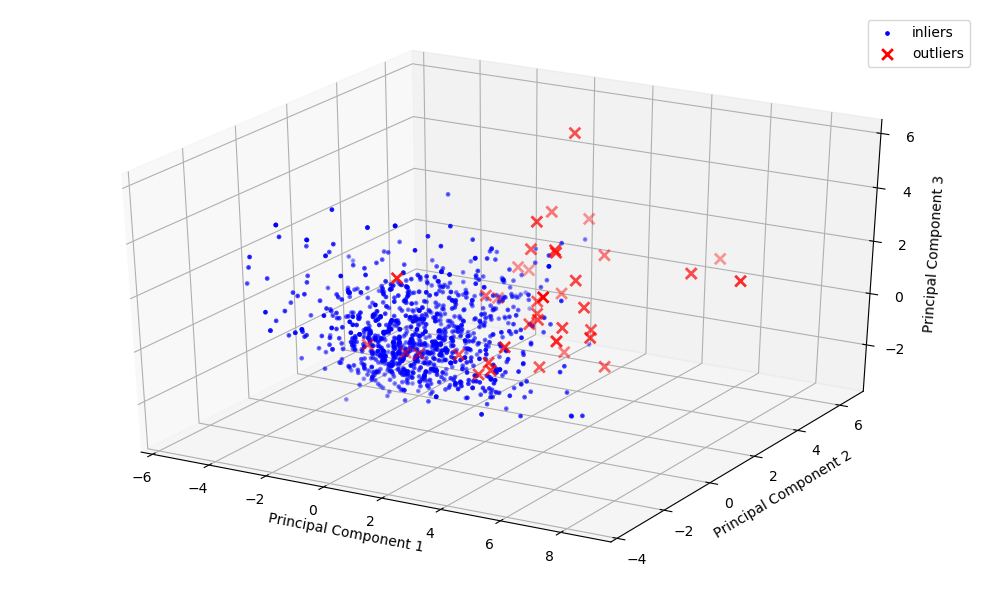
\includegraphics[angle=0,width=130mm]{../output/outlierPCA_3D_ell.png}
 \caption{
   The projection of the wines dataset onto the first three principal components with
   inlier data marked as blue circles and outliers as red x's. The
   \texttt{sklearn.covariance.EllipticalEnvelope} algorithm was used to determine the
   outliers. The contamination fraction was $0.04$. Plot idea from \citealp{Sawtelle_2017}.
 \label{FIG-Ell-Outliers-PCA-3D}}
 \end{figure}

 %%%%%%%%%%%%%%%%%%%%%%%% FIG-iForest-Outliers-PCA-3D %%%%%%%%%%%%%%%%%%%%%%%%
 \begin{figure}
 \centering 
 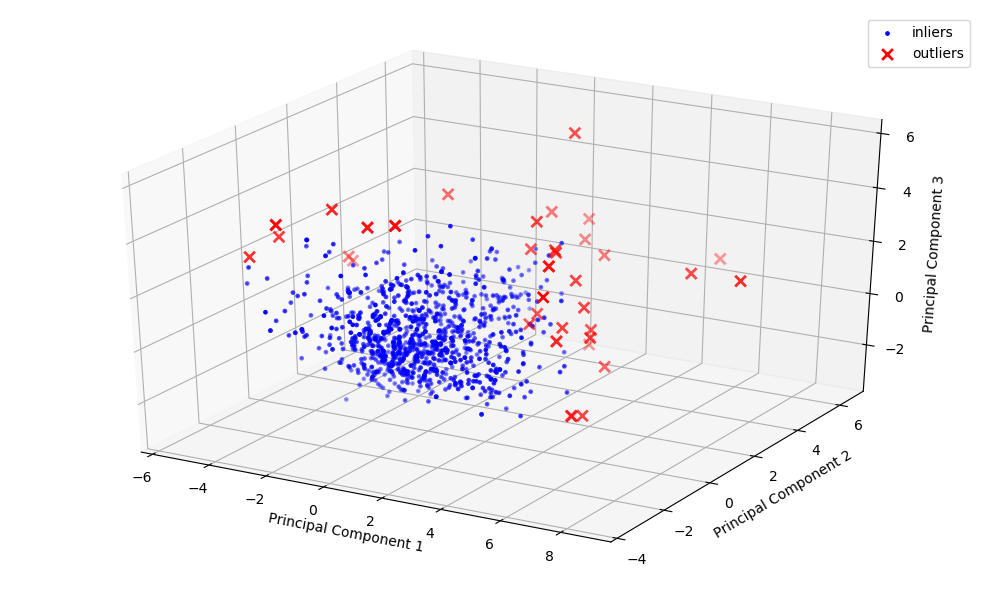
\includegraphics[angle=0,width=130mm]{../output/outlierPCA_3D_iforest.png}
 \caption{
   The projection of the wines dataset onto the first three principal components with
   inlier data marked as blue circles and outliers as red x's. The
   \texttt{sklearn.ensemble.IsolationForest} algorithm was used to determine the
   outliers. The contamination fraction was $0.04$. Plot idea from \citealp{Sawtelle_2017}.
 \label{FIG-iForest-Outliers-PCA-3D}}
 \end{figure}


 \section{Application of machine learning classifiers \label{classifiers}}

 We now look at the how a suite of machine learning classifiers
performs on the red wine dataset. To prepare the data, we first split
the data into training and test sets ($2/3$ training, $1/3$
testing). This is done randomly with
\texttt{sklearn.model\_selection.train\_test\_split}. We next apply a
scaler to the data with \texttt{sklearn.preprocessing.StandardScaler},
which standardizes the data. We train each classifier on the scaled
data set, and test the trained model on the test data. The performance
of a classifier is measured by the accuracy
(\texttt{sklearn.metrics.accuracy\_score}), the confusion matrix
(\texttt{sklearn.metrics.confusion\_matrix}), and by the average of a
5-fold cross validation
(\texttt{sklearn.model\_selection.cross\_val\_score}). The classifiers
we used for this project were: \texttt{Logistic regression},
\texttt{Decision tree}, \texttt{Random forest}, \texttt{Adaboost},
\texttt{Gradient boosting}, \texttt{Linear SVM}, and \texttt{SVM with
RBF kernel}.

The performance of the classifiers can be found in
\texttt{classifier\_performance.dat}. For each model, we vary one of
its hyperparameters. The best performing classifier is the Random
forest with \texttt{max\_depth} = 150 and \texttt{n\_estimators} =
300. Its average cross validation accuracy score was $\sim 0.673$ and
the accuracy score was $0.652$.

\subsection{Outliers}

In Section~\ref{outlier} we discussed the Elliptical Envelope and
Isolation Forest algorithms for outlier detection. We concluded, based
on the distributions of outliers in
Figures~\ref{FIG-Ell-Outliers-PCA-3D} and
\ref{FIG-iForest-Outliers-PCA-3D}, that the Isolation Forest algorithm
is the superior method for our dataset. We now measure the performance
of the Random Forest classifier on the dataset with the outliers
detected by the Isolation Forest removed from the training set. The
document which contains the performance information of the machine
learning classifiers with outliers removed is
\texttt{classifier\_performance\_no\_outliers.dat}. The best
performing classifier is the Random Forest with \texttt{max\_depth} =
100 and \texttt{n\_estimators} = 300.  The accuracy score for this
classifier is $\sim 0.669$. We do not report the average
cross-validation because the removal of the outliers likely biases the
result.

% The accuracy % score is a slightly better than the performance of
the Random Forest % on the dataset that includes the outliers.


\begin{thebibliography}{}

\bibitem[Cortez et al. 2009]{Cortez_etal_2009} Cortez, P., Cerdeira, A.,
  Almeida, F., Matos, T., \& Reis, J., Modeling wine preferences by
  data mining from physicochemical properties, In Decision Support
  Systems, Elsevier, 47(4):547-553, 2009.


\bibitem[Pedregosa et al. 2011]{Pedregosa_etal_2011} Pedregosa, F.,
  Varoquaux, G., Gramfort, A., Michel, V., Thirion, B., Grisel, O.,
  Blondel, M.,  Prettenhofer, P., Weiss, R., Dubourg, V., Vanderplas, J.,
  Passos, A., Cournapeau, D., Brucher, M., Perrot, M., Duchesnay, E.,
  Journal of Machine Learning Research, 12, 2825--2830, 2011.


\bibitem[Li 2017]{Li_2017} Li, Susan, Predict Employee Turnover With Python,
  Towards Data Science, https://towardsdatascience.com/predict-employee-turnover-with-python-da4975588aa3.

\bibitem[K Hong ]{Hong} Hong K, SCIKIT-LEARN : DATA COMPRESSION VIA DIMENSIONALITY REDUCTION I - PRINCIPAL COMPONENT ANALYSIS (PCA), BogoToBogo.com

\bibitem[Raschka 2015]{Raschka_2015} Raschka, Sebastian, Principal Component Analysis
in 3 Simple Steps, sebastianraschka.com

\bibitem[Liu et al. 2008]{Liu_etal_2008} Liu, F.T., Ting, K.M.,
  \& Zhou, Z-.H., ICDM08, 413-422, 2008.

\bibitem[Sawtelle 2017]{Sawtelle_2017} Sawtelle, S., http://sdsawtelle.github.io,
  Anomaly Detection in Scikit-Learn, 2017.
  

\end{thebibliography}


\end{document}


